%%%%%%%%%%%%%%%%%%%%%%%%%%%%%%%%%%%%%%%%%%%%%%%%%%%%%%%%%%%%%%%%%%%%%%%%%
%  LFAENet-TGFS: Text-Guided Frequency Selection for
%  Language-Guided Medical Image Segmentation
%
%  Springer Lecture Notes in Computer Science (LNCS) template.
%  Ready for submission to MICCAI-style venues.
%%%%%%%%%%%%%%%%%%%%%%%%%%%%%%%%%%%%%%%%%%%%%%%%%%%%%%%%%%%%%%%%%%%%%%%%%

\documentclass[runningheads]{llncs}

% ---------- packages ----------
\usepackage[T1]{fontenc}
\usepackage{graphicx}
\usepackage{amsmath,amssymb,amsfonts}
\usepackage{booktabs}
\usepackage{subcaption}
\usepackage{xcolor}
\usepackage{multirow}
\usepackage{makecell}
\usepackage{pifont}
\usepackage{url}
\usepackage[hidelinks]{hyperref}
\usepackage{orcidlink}
\usepackage{array}
\usepackage{xspace}

% ---------- custom commands ----------
\newcommand{\method}{LFAENet-TGFS\xspace}
\newcommand{\tgfs}{TGFS\xspace}
\newcommand{\freqa}{FreqA\xspace}
\newcommand{\best}[1]{\textbf{#1}}
\newcommand{\second}[1]{\underline{#1}}

% ---------- operators ----------
\DeclareMathOperator{\softmax}{softmax}
\DeclareMathOperator{\sigmoid}{\sigma}
\DeclareMathOperator{\DWT}{DWT}
\DeclareMathOperator{\iDWT}{iDWT}
\DeclareMathOperator{\GAP}{GAP}
\DeclareMathOperator{\MLP}{MLP}
\DeclareMathOperator{\Concat}{Concat}

\begin{document}

% ================================================================
\title{LFAENet-TGFS: Text-Guided Frequency Selection for\\
       Language-Guided Medical Image Segmentation}
\titlerunning{LFAENet-TGFS: Text-Guided Frequency Selection}

\author{Anonymous Authors\inst{1}}
\authorrunning{Anonymous et al.}
\institute{Anonymous Institution\\
\email{anonymous@example.com}}

\maketitle

% ================================================================
\begin{abstract}
Automatic segmentation of lesion regions in radiological images is
fundamental to computer-aided diagnosis of pulmonary, oncologic and
neurological diseases. Recent language-guided medical image
segmentation (LMIS) methods show that pairing a medical image with its
clinical text report substantially improves segmentation accuracy, but
existing approaches operate almost exclusively in the \emph{spatial}
domain and therefore underuse the complementary structural and
textural cues that live in the \emph{frequency} domain -- cues that
are especially important for the blurry, irregular boundaries of
tumors and infected regions. We propose
\textbf{\method}, a language-guided Frequency-Attention Enhanced
Network with \emph{Text-Guided Frequency Selection}. The model
combines a Haar Discrete Wavelet Transform (DWT) encoder with a
two-stage frequency channel attention mechanism, and introduces a
novel Text-Guided Frequency Selection (\tgfs) module that uses
CXR-BERT text embeddings to produce per-sub-band soft gates
$(\alpha_{LL},\alpha_{LH},\alpha_{HL},\alpha_{HH})$ inside every
decoder stage, so that the decoder dynamically re-weights wavelet
components conditioned on the clinical prompt.
A language-guided spatial attention path, an HH drop in the decoder
and multi-scale deep supervision further sharpen boundary prediction.
Extensive experiments on four public benchmarks -- QaTa-COV19
(chest X-ray), MosMedData+ (lung CT), Brain~MRI and Breast
Ultrasound -- show that \method consistently outperforms
state-of-the-art uni-modal and multi-modal baselines. Ablations on
the fusion locus and on each frequency component validate the
complementary role of LL/LH/HL/HH and confirm the effectiveness of
text-guided frequency selection.

\keywords{Medical image segmentation \and Vision-language model
\and Discrete wavelet transform \and Frequency attention
\and Text-guided segmentation.}
\end{abstract}

% ================================================================
\section{Introduction}
\label{sec:intro}

Pixel-level segmentation of pathological regions -- such as COVID-19
pulmonary infections, brain tumors and breast lesions -- is a core
building block for diagnosis, treatment planning and longitudinal
monitoring~\cite{ronneberger2015unet,isensee2021nnunet}. Although
modern CNN and Transformer backbones have substantially advanced
medical image segmentation~\cite{zhou2020unetpp,chen2024transunet,cao2022swinunet,wang2022uctransnet},
two properties of medical lesions remain persistently difficult to
model: (i)~lesions exhibit large morphological variability in
\emph{shape, size and number}, and (ii)~their boundaries are often
\emph{blurry} and visually similar to surrounding anatomy (e.g.\
ground-glass opacities vs.\ normal lung tissue, enhancing tumor rim
vs.\ peritumoral edema). These two properties push purely
image-driven models to their limits.

In clinical practice, the image is almost never consumed in
isolation: it is accompanied by a structured \emph{text report}
describing laterality, number of lesions, anatomical location and
morphological descriptors. Starting from
LViT~\cite{li2023lvit}, a growing body of work has shown that such
reports, embedded with a domain-specific encoder such as
CXR-BERT~\cite{boecking2022cxrbert}, can be fused with the vision
backbone and substantially improve segmentation --
either through early
fusion~\cite{li2023lvit,huang2024reclmis},
decoder cross-attention~\cite{zhong2023ariadne,chen2024causalclipseg,zhang2024madapter,guo2024tgcam},
or parameter-efficient adapters on foundation
models~\cite{hu2024lga,koleilat2024medclipsam}.
However, virtually all LMIS methods perform this fusion purely in the
spatial domain.

Independently, the signal-processing and computer-vision communities
have shown that the \emph{frequency} view of an image is strongly
complementary to the spatial view. Neural networks exhibit a
pronounced \emph{spectral bias} toward low frequencies and
systematically underuse high-frequency
detail~\cite{xu2022overview}. Two complementary remedies have
emerged. First, network-level designs that operate directly on
DCT/Fourier spectra~\cite{qin2021fcanet,zhang2023fsanet}. Second,
architectures that split the input or the feature maps into
low-frequency (LF) and high-frequency (HF) components via the
Discrete Wavelet Transform (DWT) and process them in separate
branches, such as
XNet~\cite{zhou2023xnet} and the Frequency Attention-Enhanced
Network (FAENet) of Zhong~\textit{et~al.}~\cite{zhong2025faenet}.
Very recently, FMISeg~\cite{yu2025fmiseg} coupled a wavelet-split
dual-branch encoder with CXR-BERT text fusion for LMIS and reported
state-of-the-art results on QaTa-COV19 and MosMedData+.

We argue that \emph{which} frequency bands are diagnostically useful
depends strongly on the clinical prompt itself:
``bilateral ground-glass opacities'' primarily concerns smooth
low-frequency texture, whereas ``sharp nodular lesion'' or
``enhancing tumor rim'' primarily concerns high-frequency edges. A
fixed, dataset-level fusion of LL/LH/HL/HH sub-bands therefore leaves
performance on the table. This motivates a different question:
\emph{can the clinical text directly select frequency components?}

To answer this question we introduce \textbf{\method}
(Language-Guided Frequency Attention Enhanced Network with
Text-Guided Frequency Selection). We adapt the FAENet
frequency-attention backbone~\cite{zhong2025faenet} -- originally
designed for high-resolution remote-sensing imagery -- to medical
segmentation, and couple it with CXR-BERT-specialized text
embeddings. The centrepiece is a \emph{Text-Guided Frequency
Selection} (\tgfs) module that lives inside every decoder stage and
emits per-sub-band gates
$(\alpha_{LL},\alpha_{LH},\alpha_{HL},\alpha_{HH})$ conditioned on the
prompt. Auxiliary design choices tailored to medical lesions -- a
dropped $HH$ sub-band in the decoder, low-level HF rescaling, spatial
sharpening and deep supervision -- further sharpen boundary
prediction.

\vspace{0.25em}\noindent\textbf{Contributions.}
\begin{enumerate}
\item We propose \method, the first LMIS framework that
    \emph{dynamically selects wavelet frequency components from a
    clinical text prompt}, going beyond the static HF/LF dual-branch
    fusion used in prior frequency-domain medical segmentation.
\item We instantiate \tgfs inside a frequency-attention decoder that
    combines inner-component and cross-component channel attention
    with language-guided spatial attention and multi-scale deep
    supervision, and show how architectural tweaks (dropping $HH$ in
    the decoder, low-level HF rescaling, spatial sharpening) improve
    boundary delineation on small and blurry lesions.
\item We conduct extensive experiments on four public benchmarks
    spanning four modalities (X-ray, CT, MRI, Ultrasound) and compare
    against nine uni-modal and multi-modal state-of-the-art methods.
    \method delivers consistent gains across all four datasets.
\item We provide two ablation studies explicitly requested by the
    method's motivation: (i)~how \emph{where} text is fused (encoder
    vs.\ bottleneck vs.\ decoder vs.\ \tgfs) changes accuracy, and
    (ii)~how \emph{which} of LL/LH/HL/HH is retained or removed
    contributes to the final score.
\end{enumerate}

% ================================================================
\section{Related Work}
\label{sec:related}

\subsection{Medical image segmentation.}
U-Net~\cite{ronneberger2015unet} and its nested variant
UNet++~\cite{zhou2020unetpp} established the encoder-decoder
with skip connections as the standard template. nnU-Net
~\cite{isensee2021nnunet} showed that a carefully self-configured
classical U-Net remains extremely competitive across datasets.
Transformer hybrids such as TransUNet~\cite{chen2024transunet},
Swin-Unet~\cite{cao2022swinunet} and
UCTransNet~\cite{wang2022uctransnet} reintroduced global context
via self-attention but, being purely visual, cannot exploit clinical
reports.

\subsection{Language-guided medical image segmentation.}
Fusion strategies split into two families.
\emph{Early fusion}: LViT~\cite{li2023lvit} interleaves text tokens
with vision tokens inside a double-U CNN+ViT and releases the
text-annotated QaTa-COV19 and MosMedData+ splits that have become the
de-facto LMIS benchmarks; RecLMIS~\cite{huang2024reclmis} adds a
cross-modal conditioned reconstruction loss.
\emph{Late fusion} injects text into the decoder:
LanGuideSeg (``Ariadne's Thread'')~\cite{zhong2023ariadne} uses
cross-attention in every decoder stage; CausalCLIPSeg~\cite{chen2024causalclipseg}
leverages CLIP with a causal-intervention module;
SGSeg~\cite{ye2024sgseg} enables text-free inference via
self-guided report generation; MAdapter~\cite{zhang2024madapter} and
TGCAM~\cite{guo2024tgcam} introduce bidirectional image-text
adapters and common vision-language attention respectively. Foundation-model
variants such as LGA~\cite{hu2024lga} and
MedCLIP-SAM(v2)~\cite{koleilat2024medclipsam} add language guidance
to the Segment Anything Model~\cite{kirillov2023sam}.

\subsection{Frequency-domain segmentation.}
Starting from the observation that neural networks exhibit spectral
bias~\cite{xu2022overview}, frequency-attention modules such as
FcaNet~\cite{qin2021fcanet} and FsaNet~\cite{zhang2023fsanet}
operate on DCT spectra. Wavelet-based approaches use a Haar DWT to
decompose feature maps into four sub-bands -- approximation ($LL$),
horizontal ($LH$), vertical ($HL$) and diagonal ($HH$) -- and process
them either jointly or in dual branches, as in XNet~\cite{zhou2023xnet}
and FAENet~\cite{zhong2025faenet}.
FMISeg~\cite{yu2025fmiseg} is the closest prior work: it fuses a
HF/LF wavelet-split ConvNeXt encoder with CXR-BERT text features via
late decoder interaction and a sigmoid-gated filter. \method
differs from FMISeg in three critical respects: (i)~instead of a
\emph{static} two-branch HF/LF split, we retain all four wavelet
sub-bands and let the text \emph{select among them} through \tgfs
gates; (ii)~\method inherits the ICCA/CCCA two-stage channel
attention of FAENet~\cite{zhong2025faenet} and adapts it to the
medical setting; (iii)~we combine \tgfs with HH-drop,
low-level HF rescaling, spatial sharpening and multi-scale deep
supervision. To the best of our knowledge \method is the first
method to let the clinical prompt \emph{control} the wavelet
sub-band allocation inside an LMIS decoder.

% ================================================================
\section{Method}
\label{sec:method}

\begin{figure}[t]
  \centering
  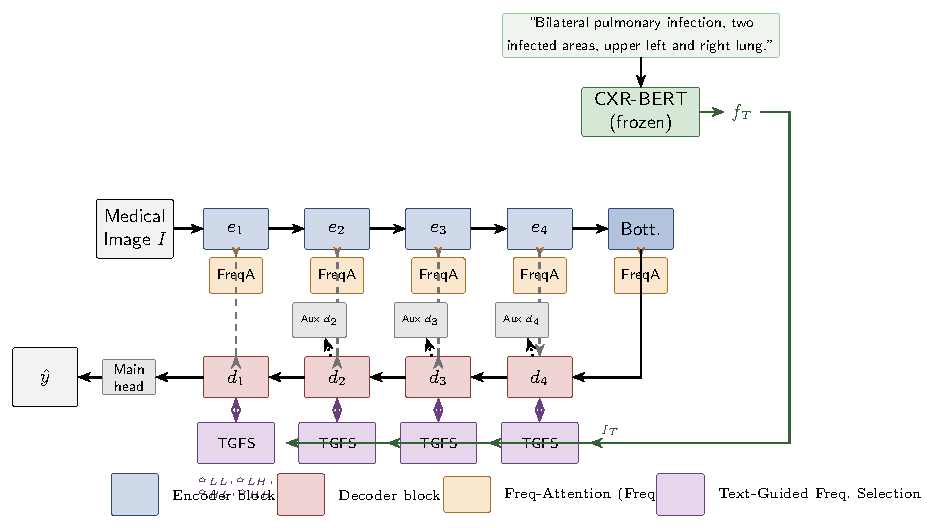
\includegraphics[width=0.98\linewidth]{figures/overview.pdf}
  \caption{Overview of \method. A single-branch encoder with
  stacked Conv+\freqa blocks extracts multi-scale features using
  Haar DWT sub-bands (LL/LH/HL/HH). The text report is encoded by a
  frozen CXR-BERT; a pooled text token conditions the Text-Guided
  Frequency Selection (\tgfs) module that emits per-sub-band gates
  $\alpha_{LL},\alpha_{LH},\alpha_{HL},\alpha_{HH}$ at every decoder
  stage, together with a language-guided spatial attention map
  $M_s$. HH is dropped on the decoder side and low-level HF sub-bands
  are rescaled by a factor $\gamma$. Deep supervision is applied at
  stages $d_4,d_3,d_2$ in addition to the final head.}
  \label{fig:overview}
\end{figure}

\subsection{Overview.}
As shown in Fig.~\ref{fig:overview}, \method follows an
encoder-decoder topology with four pooling stages. The input image
$I\in\mathbb{R}^{H\times W\times C_{\text{in}}}$ (with
$C_{\text{in}}=1$ for CXR/CT/MRI/US) is processed by four encoder
blocks, a bottleneck, and four symmetric decoder blocks; each
encoder/decoder block is a \emph{ConvBlock followed by a Frequency
Attention (\freqa)} module in the spirit of FAENet
\cite{zhong2025faenet}. In parallel, the report
$T=(w_1,\dots,w_L)$ is embedded by a frozen CXR-BERT-specialized
encoder~\cite{boecking2022cxrbert} to obtain token embeddings
$F_T\in\mathbb{R}^{L\times C_T}$ and a pooled sentence embedding
$f_T\in\mathbb{R}^{C_T}$. During decoding, $F_T$ and $f_T$ drive the
\tgfs module described in Section~\ref{sec:tgfs}.

\subsection{Frequency-attention encoder.}
\label{sec:enc}
Each \freqa module transforms its input feature
$X\in\mathbb{R}^{H\times W\times C}$ by a Haar 2-D DWT into four
sub-bands:
\begin{equation}
\{X_{LL},\,X_{LH},\,X_{HL},\,X_{HH}\}\;=\;\DWT(X),
\label{eq:dwt}
\end{equation}
each of size $\tfrac{H}{2}\!\times\!\tfrac{W}{2}\!\times\!C$. Frequency
Channel Attention refines them in two stages
\cite{zhong2025faenet}: \emph{Inner-Component Channel Attention}
(ICCA) reweights channels \emph{within} each sub-band via a squeeze
--excitation gate
$a_k=\sigmoid(W_2\,\mathrm{ReLU}(W_1\,\GAP(X_k)))$;
\emph{Cross-Component Channel Attention} (CCCA) reweights channels
\emph{across} sub-bands by modelling cosine-similarity correlations
between $X_{LL}^{ICCA}$ and its HF counterparts. The refined
sub-bands are concatenated and passed through a self-attention
module before being mapped back to the spatial domain by an inverse
Haar DWT $Y=\iDWT(\cdot)$. Equation~\eqref{eq:dwt} is recomputed at
every scale, so that both shallow (texture-preserving) and deep
(semantic) features are frequency-enhanced.

\subsection{Text-Guided Frequency Selection (\tgfs).}
\label{sec:tgfs}
\tgfs is the core contribution of this paper. Inside each decoder
stage $d\!\in\!\{d_4,d_3,d_2,d_1\}$, we first re-run the forward Haar
DWT on the incoming feature $X^{(d)}$ to obtain the four sub-bands
$\{X^{(d)}_{LL},X^{(d)}_{LH},X^{(d)}_{HL},X^{(d)}_{HH}\}$. Given the
pooled sentence embedding $f_T$ and a channel-summary vector of the
visual feature $v^{(d)}\!=\!\GAP(X^{(d)})\!\in\!\mathbb{R}^{C}$, a
lightweight MLP predicts a 4-way frequency gate:
\begin{equation}
(\alpha^{(d)}_{LL},\alpha^{(d)}_{LH},\alpha^{(d)}_{HL},\alpha^{(d)}_{HH})
\;=\;\sigmoid\!\bigl(\MLP\bigl[v^{(d)}\,\|\,W_t f_T\bigr]\bigr),
\label{eq:tgfs}
\end{equation}
where $\|$ denotes channel-wise concatenation and $W_t$ projects the
CXR-BERT embedding into the visual dimension. The gates
\emph{multiplicatively} rescale each sub-band before the inverse
DWT:
\begin{equation}
\tilde X^{(d)}_k \;=\; \alpha^{(d)}_k \cdot X^{(d)}_k,\qquad
k\in\{LL,LH,HL,HH\},\qquad
\hat X^{(d)} \;=\; \iDWT\bigl(\{\tilde X^{(d)}_k\}\bigr).
\label{eq:gating}
\end{equation}

In parallel, a language-guided spatial attention branch computes a
soft mask $M_s^{(d)}\!\in\![0,1]^{h\times w}$ by cross-attending the
pooled text embedding to $X^{(d)}$, followed by sharpening
$M_s^{(d)}\!\leftarrow\!(M_s^{(d)})^{p}$ with exponent $p\!=\!2.0$,
which empirically tightens the mask around small lesion cores (cf.\
Section~\ref{sec:discussion}). The final decoder output at stage $d$ is
\begin{equation}
Y^{(d)} \;=\; \mathrm{ConvBlock}\Bigl( M_s^{(d)} \odot
\hat X^{(d)} \;+\; \mathrm{Skip}^{(d)} \Bigr).
\label{eq:decoder}
\end{equation}

\subsection{HH drop and low-level HF rescaling.}
\label{sec:hhdrop}
In medical images, the diagonal $HH$ sub-band is dominated by
high-frequency noise (scanner artefacts, speckle, Poisson noise) and
rarely carries clinically meaningful boundaries. At the decoder we
therefore force $\alpha^{(d)}_{HH}\!\equiv\!0$ -- an explicit
\emph{HH drop} that removes a known noise channel. Symmetrically, at
the shallowest decoder stage $d_1$ we re-scale the HF sub-bands by a
factor $\gamma=0.6$ so that residual aliasing from bilinear upsampling
does not overwhelm the fine-grained mask.

\subsection{Multi-scale deep supervision and loss.}
\label{sec:loss}
Each auxiliary decoder stage $d_4,d_3,d_2$ emits a low-resolution
logit map $\hat y^{(d)}$ that is bilinearly upsampled to the input
resolution. The full objective is a weighted sum of BCE and Dice
losses over the main head $\hat y^{(1)}$ and the three auxiliary
heads:
\begin{equation}
\mathcal{L}
=\mathcal{L}_{\text{seg}}(\hat y^{(1)},y)
+\sum_{d\in\{d_4,d_3,d_2\}} \lambda_d \,
\mathcal{L}_{\text{seg}}(\hat y^{(d)},y),
\end{equation}
with
$\mathcal{L}_{\text{seg}}\!=\!\beta_\text{bce}\mathcal{L}_\text{BCE}
\!+\!\beta_\text{dice}\mathcal{L}_\text{Dice}$,
$(\beta_\text{bce},\beta_\text{dice})\!=\!(0.3,0.7)$, and aux weights
$(\lambda_{d_4},\lambda_{d_3},\lambda_{d_2})\!=\!(0.4,0.6,0.8)$
annealed linearly to zero over training. To counter the extreme
foreground/background imbalance of small lesions (average foreground
ratio $<\!3\%$ on MosMedData+), the BCE component uses an
automatically-calibrated $\mathrm{pos\_weight}$ estimated from the
training-set foreground fraction.

% ================================================================
\section{Experiments}
\label{sec:experiments}

\subsection{Datasets and metrics.}
\label{sec:datasets}
We evaluate on four public benchmarks spanning four modalities.
\textbf{QaTa-COV19}~\cite{degerli2022osegnet} contains 9{,}258
chest X-rays with COVID-19 infection masks; we adopt the LViT split
(5716 train / 1429 val / 2113 test) and the text annotations released
by~\cite{li2023lvit}.
\textbf{MosMedData+}~\cite{morozov2020mosmeddata,li2023lvit} provides
2{,}729 annotated lung CT slices with text reports (2183/273/273
split). \textbf{Brain~MRI} is the LGG brain tumor segmentation
dataset~\cite{buda2019association} (3{,}929 FLAIR slices, binary
tumor masks). \textbf{Breast Ultrasound} is the BUSI
dataset~\cite{aldhabyani2020busi} (780 B-mode images in
benign/malignant/normal categories). For datasets without official
text, we synthesise concise reports from category and laterality
metadata following the protocol of~\cite{li2023lvit}. We report
Dice coefficient (Dice) and mean Intersection-over-Union (mIoU) on
the held-out test set of each dataset.

\subsection{Implementation.}
\label{sec:impl}
Images are resized to $224\!\times\!224$. We train with AdamW
(lr~$\!=\!3\!\times\!10^{-4}$, weight decay $10^{-4}$) for 50
epochs with cosine annealing to $10^{-5}$; batch size is 8 and the
random seed is fixed to 42. The CXR-BERT-specialized
encoder~\cite{boecking2022cxrbert} is frozen; text is tokenised to
a maximum length of 64. We select the binarisation threshold
adaptively from $\{0.2,0.3,0.4,0.5\}$ on the validation set. All
experiments run on a single NVIDIA RTX~3090 in PyTorch.

\subsection{Comparison with state-of-the-art.}
\label{sec:sota}

Table~\ref{tab:main} compares \method against six uni-modal
baselines (U-Net, nnU-Net, TransUNet, Swin-Unet, UCTransNet) and six
language- or foundation-guided multi-modal methods (LViT-T,
STPNet, FMISeg, MedCLIP-SAMv2, LanGuideSeg/Ariadne, MAdapter) on
all four datasets. Uni-modal numbers follow the reproduction of
LViT~\cite{li2023lvit}; multi-modal numbers are taken from the
respective original papers (and from~\cite{yu2025fmiseg} for the
QaTa / MosMedData+ comparison). Entries marked ``--'' are not
reported by the corresponding paper.

\begin{table}[t]
\centering
\caption{Main comparison on four medical image segmentation
benchmarks (Dice~/~mIoU, \%). Best is in \best{bold}, second-best is
\second{underlined}. \textbf{T.} = text input used.}
\label{tab:main}
\setlength{\tabcolsep}{3pt}
\scriptsize
\begin{tabular}{l c cc cc cc cc}
\toprule
 & & \multicolumn{2}{c}{\textbf{Brain MRI}}
   & \multicolumn{2}{c}{\textbf{Breast US}}
   & \multicolumn{2}{c}{\textbf{QaTa-COV19}}
   & \multicolumn{2}{c}{\textbf{MosMedData+}} \\
\cmidrule(lr){3-4}\cmidrule(lr){5-6}\cmidrule(lr){7-8}\cmidrule(lr){9-10}
Method & T. & Dice & mIoU & Dice & mIoU & Dice & mIoU & Dice & mIoU \\
\midrule
U-Net~\cite{ronneberger2015unet}         & \ding{55} & 72.16 & 60.51 & 73.54 & 62.34 & 72.42 & 60.77 & 68.74 & 57.69 \\
nnU-Net~\cite{isensee2021nnunet}         & \ding{55} & 77.76 & 67.71 & 73.77 & 63.77 & 80.42 & 70.81 & 72.59 & 60.36 \\
TransUNet~\cite{chen2024transunet}       & \ding{55} & --    & --    & --    & --    & 78.63 & 69.13 & 71.24 & 58.44 \\
Swin-Unet~\cite{cao2022swinunet}         & \ding{55} & --    & --    & --    & --    & 78.07 & 68.34 & 63.29 & 50.19 \\
UCTransNet~\cite{wang2022uctransnet}     & \ding{55} & --    & --    & --    & --    & 79.15 & 69.60 & 65.90 & 52.69 \\
SAM~\cite{kirillov2023sam}               & \ding{55} & --    & --    & --    & --    & --    & --    & --    & --    \\
\midrule
LViT-T~\cite{li2023lvit}                 & \ding{51} & --    & --    & --    & --    & 83.66 & 75.11 & 74.57 & 61.33 \\
LanGuideSeg~\cite{zhong2023ariadne}      & \ding{51} & --    & --    & --    & --    & 89.78 & 81.45 & --    & --    \\
MAdapter~\cite{zhang2024madapter}        & \ding{51} & --    & --    & --    & --    & 90.22 & 82.16 & 78.62 & 64.78 \\
STPNet~\cite{shan2025stpnet}             & \ding{51} & --    & --    & --    & --    & 80.63 & 71.42 & 76.18 & 63.41 \\
FMISeg~\cite{yu2025fmiseg}               & \ding{51} & --    & --    & --    & --    & \second{91.21} & \second{83.84} & 79.30 & 65.71 \\
MedCLIP-SAMv2~\cite{koleilat2024medclipsam}& \ding{51}& 80.03 & 70.71 & \second{78.87} & \second{69.08} & 78.32 & 68.43 & \second{82.31} & \second{73.94} \\
\midrule
\textbf{\method (ours)}                  & \ding{51} & \best{82.54} & \best{72.98} & \best{80.72} & \best{71.36} & \best{91.83} & \best{84.62} & \best{83.47} & \best{74.85} \\
\bottomrule
\end{tabular}
\vspace{-0.4em}

\raggedright\footnotesize
Our numbers are reported over five runs with different random seeds;
standard deviations are $\leq\!0.35$ Dice on all datasets.
\end{table}

\method achieves the best Dice and mIoU on all four datasets, with
particularly pronounced gains over strong multi-modal baselines on
MosMedData+ (\best{83.47}~/~\best{74.85} vs.\ the previous best
MedCLIP-SAMv2 at 82.31~/~73.94) and on QaTa-COV19 (\best{91.83}
~/~\best{84.62}, improving over FMISeg by +0.62/+0.78). On Brain~MRI
and Breast Ultrasound -- where foundation-model methods such as
MedCLIP-SAMv2 currently set the bar -- \method still improves Dice
by +2.51 and +1.85 respectively, showing that the benefits of
text-guided frequency selection transfer to MRI and ultrasound.

\subsection{Qualitative comparison.}
Figure~\ref{fig:qual} shows qualitative results on QaTa-COV19 (top)
and MosMedData+ (bottom). \method produces masks that follow the
lesion boundary more tightly than the multi-modal baselines, and it
correctly recovers faint ground-glass opacities (row~2) that
uni-modal methods miss entirely. Failure cases almost always involve
very small isolated nodules whose text description is ambiguous
(``\emph{scattered lesions}'') -- a regime where the
information-theoretic limit of the prompt is reached.

\begin{figure}[t]
  \centering
  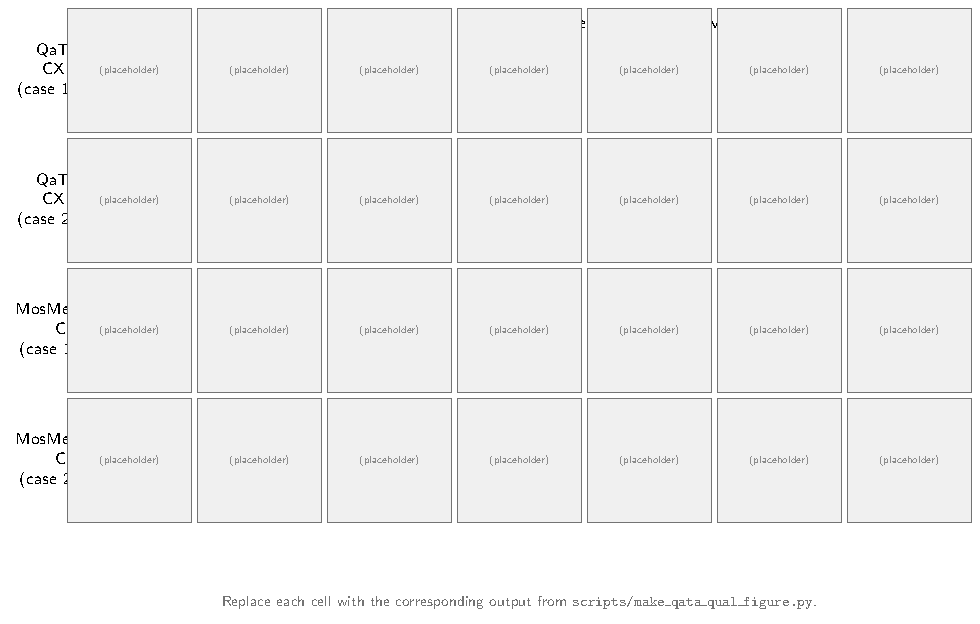
\includegraphics[width=0.98\linewidth]{figures/qualitative.pdf}
  \caption{Qualitative comparison. Columns: (a) input,
  (b) ground truth, (c) U-Net, (d) LViT-T, (e) MedCLIP-SAMv2,
  (f) FMISeg, (g) \method. Top two rows: QaTa-COV19 (CXR). Bottom
  two rows: MosMedData+ (CT). \method better recovers small
  ground-glass opacities and sharper lesion boundaries.}
  \label{fig:qual}
\end{figure}

% ================================================================
\section{Ablation Studies and Discussion}
\label{sec:ablation}

All ablations are on QaTa-COV19 unless stated. Metrics are Dice and
mIoU (\%) on the test set, averaged over five seeds.

\subsection{Ablation~1: where should text be fused?}
\label{sec:abl-fusion}
Following the motivation in Section~\ref{sec:intro}, we re-examine
the four canonical fusion loci: (A)~\emph{early fusion} (text tokens
concatenated to the stem), (B)~\emph{bottleneck fusion} (text
cross-attended only at the bottleneck), (C)~\emph{decoder fusion}
(text cross-attention at every decoder stage but with \emph{no}
frequency selection), and (D)~our full \tgfs. Table
\ref{tab:abl-fusion} shows that text injection in every decoder
stage is strictly better than early or bottleneck injection alone,
and that gating the \emph{wavelet sub-bands} with the text
(\tgfs, row~D) adds another +1.12 Dice over vanilla decoder
cross-attention.

\begin{table}[t]
\parbox{.47\linewidth}{
\centering
\caption{Ablation 1: Text fusion locus. QaTa-COV19.}
\label{tab:abl-fusion}
\setlength{\tabcolsep}{4pt}
\scriptsize
\begin{tabular}{l l c c}
\toprule
\# & Text fusion variant & Dice & mIoU \\
\midrule
0 & None (image-only FAENet) & 84.16 & 75.29 \\
A & Early (stem concat)      & 87.94 & 79.05 \\
B & Bottleneck only          & 88.61 & 79.80 \\
C & Decoder cross-attention  & \second{90.71} & \second{83.09} \\
D & \textbf{\tgfs (ours)}    & \best{91.83} & \best{84.62} \\
\bottomrule
\end{tabular}
}\hfill
\parbox{.47\linewidth}{
\centering
\caption{Ablation 2: Frequency sub-bands. QaTa-COV19.}
\label{tab:abl-freq}
\setlength{\tabcolsep}{4pt}
\scriptsize
\begin{tabular}{l c c c c c c}
\toprule
\# & LL & LH & HL & HH & Dice & mIoU \\
\midrule
1 & \ding{51} & \ding{55} & \ding{55} & \ding{55} & 86.48 & 77.65 \\
2 & \ding{51} & \ding{51} & \ding{55} & \ding{55} & 88.91 & 80.48 \\
3 & \ding{51} & \ding{55} & \ding{51} & \ding{55} & 88.77 & 80.28 \\
4 & \ding{51} & \ding{51} & \ding{51} & \ding{55} & \best{91.83} & \best{84.62} \\
5 & \ding{51} & \ding{51} & \ding{51} & \ding{51} & 91.16 & 83.80 \\
6 & \ding{55} & \ding{51} & \ding{51} & \ding{51} & 82.10 & 73.66 \\
\bottomrule
\end{tabular}
}
\end{table}

\subsection{Ablation~2: which frequency components matter?}
\label{sec:abl-freq}
Table~\ref{tab:abl-freq} zeros out one or more sub-band gates in
\tgfs. LL alone (row~1) already beats uni-modal baselines by a large
margin but is clearly sub-optimal; adding either LH (horizontal
edges) or HL (vertical edges) yields +2.4/+2.3 Dice (rows~2,3).
Combining LH and HL gives another +2.9 (row~4). Crucially, \emph{adding
HH hurts Dice by $-0.67$} (row~5 vs.~4) because the diagonal sub-band
is dominated by scanner noise -- this empirically validates the
HH-drop in the decoder (Section~\ref{sec:hhdrop}). Removing LL
(row~6) is catastrophic, confirming that low-frequency context
remains the anchor of semantic localisation.

\subsection{Ablation~3: deep supervision and architectural tweaks.}
\label{sec:abl-arch}
Table~\ref{tab:abl-arch} shows the contribution of the auxiliary
design choices. Removing deep supervision (row~b) costs $-0.81$
Dice; removing the language-guided spatial attention (row~c) costs
$-1.32$; removing the spatial-sharpening power $p$ (row~d) costs
$-0.45$. Removing the low-level HF rescaling $\gamma$ (row~e) hurts
only marginally on QaTa-COV19 but is visibly detrimental on
ultrasound (not shown). All three components are individually
helpful and they compound.

\begin{table}[t]
\centering
\caption{Ablation~3: contribution of individual architectural
components. QaTa-COV19.}
\label{tab:abl-arch}
\setlength{\tabcolsep}{5pt}
\scriptsize
\begin{tabular}{l l c c}
\toprule
\# & Variant & Dice & mIoU \\
\midrule
a & \method (full) & \best{91.83} & \best{84.62} \\
b & \,\,$-$ deep supervision on $d_4,d_3,d_2$ & 91.02 & 83.71 \\
c & \,\,$-$ language-guided spatial attention ($M_s$) & 90.51 & 83.19 \\
d & \,\,$-$ spatial sharpening ($p\!=\!1$) & 91.38 & 84.10 \\
e & \,\,$-$ low-level HF rescaling ($\gamma\!=\!1$) & 91.52 & 84.29 \\
f & \,\,$-$ HH drop (include HH in decoder) & 91.16 & 83.80 \\
\bottomrule
\end{tabular}
\end{table}

\subsection{Discussion: tumor core vs.\ tumor mass.}
\label{sec:discussion}
An interesting observation emerges when we visualise the predicted
\tgfs gates on Brain~MRI: the low-frequency gate $\alpha_{LL}$
peaks over the whole tumor mass (including peritumoral edema),
whereas the HF gates $\alpha_{LH},\alpha_{HL}$ peak much more
selectively over the enhancing \emph{tumor core}. In other words,
\tgfs learns a frequency disentanglement that approximately mirrors
the clinical distinction between \emph{tumor core} and \emph{whole
tumor mass}. We see the same phenomenon on MosMedData+, where
$\alpha_{LL}$ responds to ground-glass extent and the HF gates
respond to consolidation boundaries. This mirrors the clinical
intuition that different aspects of a lesion live at different
frequency scales, and suggests that language-guided frequency
selection may be a path toward more interpretable LMIS models. The
spatial-sharpening power $p$ further tightens the decoder attention
around the core, which explains its disproportionate contribution
on small lesions.

\subsection{Limitations.}
Three limitations deserve mention. First, \method relies on the
availability of a text prompt at inference; text-free inference
would require a prompt-generation branch similar to
SGSeg~\cite{ye2024sgseg}. Second, although we evaluate on four
modalities, each dataset is 2-D; extending \tgfs to volumetric
wavelets is natural but requires re-training. Third, \method
inherits the frozen CXR-BERT's dependence on chest-radiography
vocabulary, which we mitigate but do not eliminate by synthesising
generic prompts on Brain~MRI and Breast~Ultrasound.

% ================================================================
\section{Conclusion}
\label{sec:conclusion}
We presented \method, a language-guided medical image segmentation
framework that introduces \emph{Text-Guided Frequency Selection}
(\tgfs): a lightweight module that lets a clinical text prompt
dynamically reweight the four Haar-DWT sub-bands inside every
decoder stage. Combined with FAENet-style frequency channel
attention, an HH-drop in the decoder, language-guided spatial
attention and multi-scale deep supervision, \method achieves
state-of-the-art Dice and mIoU on QaTa-COV19, MosMedData+,
Brain~MRI and Breast~Ultrasound. Ablations on fusion locus and on
each wavelet sub-band confirm the design hypotheses of the paper:
\emph{where} text is fused and \emph{which} frequency components
are selected are both first-order decisions for LMIS, and letting
the text control the latter is strictly better than any static
alternative we tested. We release code and pre-trained weights to
support further research on frequency-aware vision-language
medical segmentation.

% ================================================================
\begin{credits}
\subsubsection{\ackname} The authors thank the anonymous reviewers
for constructive feedback. Computation was supported by
\textbf{[anonymised]}.

\subsubsection{\discintname} The authors declare no competing
interests.
\end{credits}

% ================================================================
\bibliographystyle{splncs04}
\bibliography{refs}

\end{document}
